Las partículas elementales están divididas en dos categorías según el valor de su espín en \fermiones ~ (espín semi-entero, para elementales $1/2$) y \bosones ~ (espín entero, para elementales $1$ menos el higgs con $0$), estos obedecen también a la \fermidirac ~ y la \boseeinstein, respectivamente, solo cumpliendo el \pauli ~ los primeros.

El \ME ~ describe la composición de la materia bariónica usando 6 quarks, 6 leptones (fermiones) y partículas mediadoras de las interacciones fundamentales conocidas (bosones), que son los fotones $\mathbf{\gamma}$ (interacción electromagnética), los gluones $\mathbf{g}$ (interacción fuerte) y las partículas $\mathbf{W}^\pm$ y $\mathbf{Z}$ (fuerza débil). 
El bosón de Higgs $\mathbf{H}$ tiene un papel fundamental en el mecanismo de Higgs el cual dota de la propiedad de masa a las partículas elementales. Actualmente la interacción gravitacional no está descrita por algún bosón del \ME.

\begin{figure}[!b]
    \centering
    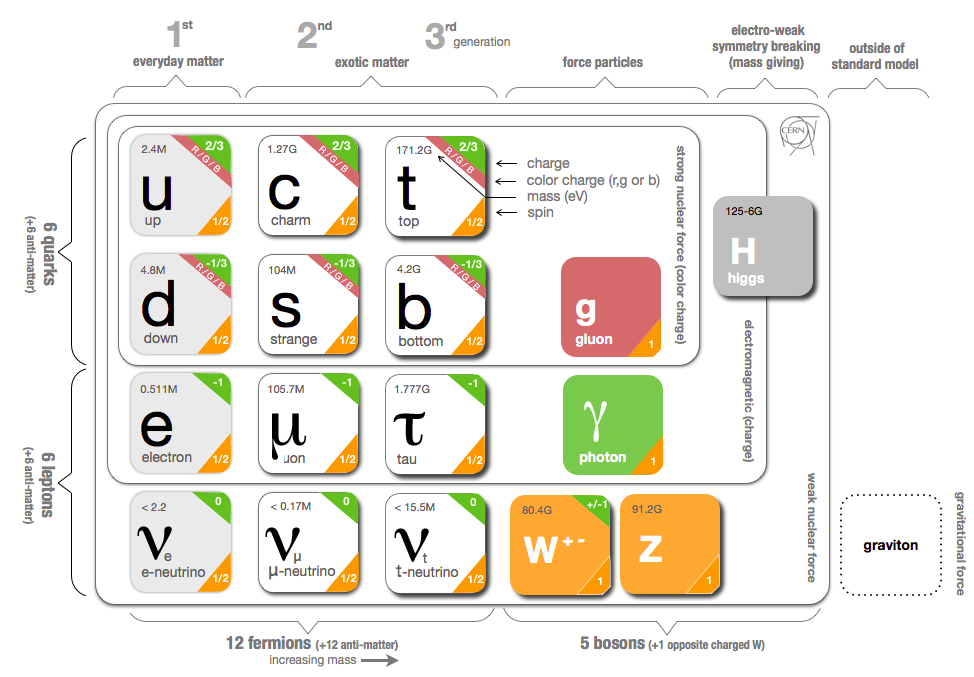
\includegraphics[width=.8\textwidth]{Fisica_de_Particulas/imagenes/standard_model.png}
    \caption{Clasificación de las partículas según el modelo estándar de las partículas elementales.}
    \label{estandar}
\end{figure}

%\subsection*{Quarks}

Los quarks Son fermiones que poseen carga eléctrica fraccionada ($- 1/3$ o $+ 2/3$) y carga de color (\textbf{R}, \textbf{G} o \textbf{B}), por lo que interactúan por medio del fotón $\gamma$ y del glúon $\mathbf{g}$. El campo de estudio dedicado a las interacciones entre quarks y gluones se llama Cromodinámica Cuántica (\QCD). Sin embargo, los quarks solo se encuentran en estados ligados llamados hadrones, ya sean bariones formados por tres quarks de diferente color (\textbf{qqq}), o mesones formado por un par quark-antiquark\footnote{Las antipartículas poseen la misma masa y espín, pero carga eléctrica contraria.} (\textbf{q\={q}}). Dado que los quarks son fermiones, dos quarks del mismo tipo no pueden tener los mismos n\'umeros cuánticos en el mismo hadrón.

En este grupo los quarks poseen carga eléctrica entera o neutra, estas son partículas indivisibles y por lo tanto elementales. Existen seis tipos como se pueden observar en la Fig. \ref{neuronas}: up $\mathbf{u}$(arriba), down $\mathbf{d}$(abajo), charm $\mathbf{c}$(encanto), strange $\mathbf{s}$(extrañeza), top $\mathbf{t}$(superior) y bottom $\mathbf{b}$(inferior). 
% ems: Nombrar los seis quarks haciendo referencia a la Fig. 1-1. Puedes poner de ejemplo a los dos bariones más conocidos: el neutrón y el protón.
Algunos ejemplos de bariones son:
\begin{itemize}
    \item \href{https://es.wikipedia.org/wiki/Bari\%C3\%B3n_omega}{\textbf{El neutrón ($N^0$) :}} es incluida en la definición de nucleones ya que conforman el núcleo de los átomos, es una partícula subatómica sin carga neta,  de la \QCD ~ se define que es partícula compuesta por la unión estable de quarks \textbf{udd}.
    \item \href{https://es.wikipedia.org/wiki/Prot\%C3\%B3n}{\textbf{El protón ($p^+$) :}} es incluida en la definición de nucleones ya que conforman el núcleo de los átomos, es una partícula subatómica con una carga eléctrica elemental positiva, de la \QCD ~ se define que es partícula compuesta por la unión estable \textbf{uud}.
\end{itemize}

Todos los hadrones tienen una respectiva antipartícula conformada por los antiquarks correspondientes.

%\subsection*{Leptones}

Los leptones forman parte de la familia de los fermiones por lo cual poseen espín semi-entero, además no poseen carga de color y por lo tanto tampoco experimentan la interacción nuclear fuerte. Se han identificado tres ``sabores`` de partículas: uno de materia ordinaria y dos de materia exótica. Al primero corresponden el electrón $e$ y el neutrino $\nu_e$ mientras que a la materia exótica corresponden el muón $\mu$ y el tauón $\tau$ con sus respectivos neutrinos $\nu_\mu$ y $\nu_\tau$ (ver Fig. \ref{estandar}).

\begin{itemize}
    \item \href{https://es.wikipedia.org/wiki/Electr\%C3\%B3n}{\textbf{El electrón :}} es una partícula elemental perteneciente a la primera generación de los leptones, representada por el símbolo $e^-$ posee una carga eléctrica elemental negativa. Su antipartícula es denominada positrón idéntica excepto por la carga de signo opuesto.
    
    \item \href{https://es.wikipedia.org/wiki/Muon}{\textbf{El muón :}} 
     es una partícula elemental masiva perteneciente a la segunda generación de leptones, representada por el símbolo $\mu^-$ su masa es 100 veces mayor que la del electrón. Su correspondiente antipartícula es el antimuón ($\mu^+$).
    
    \item \href{https://es.wikipedia.org/wiki/Tau_(part\%C3\%ADcula)}{\textbf{El tau :}} llamada a veces tauón, es una partícula elemental masiva que pertenece a la tercera generación de leptones, representada por el símbolo $\tau^-$, su masa es cerca de 3500 veces mayor que la del electrón. Su correspondiente antipartícula es el antitau o antitauón ($\tau^+$).
    
    \item \href{https://es.wikipedia.org/wiki/Neutrino}{\textbf{Los neutrinos :}}
    son partículas subatómicas sin carga y de espín $1/2$, que estas partículas tienen masa muy pequeña, su interacción con las demás partículas es mínima, por lo que pasan a través de la materia ordinaria sin apenas perturbarla. Existen tres tipos de neutrinos asociados a cada una de las familias leptónicas (o sabores): neutrino electrónico ($v_e$), neutrino muónico ($v_\mu$) y neutrino tauónico ($v_\tau$) más sus respectivas antipartículas.

\end{itemize}

Cada partícula anteriormente descrita con su correspondiente antipartícula corresponde con la composición de la materia bariónica.
